% Generated from main.typ. Typst is authoritative; regeneration overwrites this file.
\documentclass{qlnotes-export}

\title{MATH 597: Measure Theory}
\subtitle{Typst-first course notes and worked homeworks}
\author{Qiulin Fan}
\date{Winter 2025}

\begin{document}
\mainmatter
\chapter{Homework 4: on measurable functions(36/40)}\label{homework-4-on-measurable-functions3640}

\emph{None of the following questions will be graded. Do them, but do not hand them in}.

\section{One with Vitali.}

Let \((X,\mathcal{A})\) be a measurable space, and \(E \subset X\) a subset. Prove that \(E \in \mathcal{A}\) iff the function \(\chi_{E}\) is measurable. Use this to construct a function \(f:{\mathbb{R}}\rightarrow{\mathbb{R}}\) that is not Lebesgue measurable.

\section{\texorpdfstring{Truncations in \(L^{+}\): 通过 \(\int f_{n}\) 或者 \(\int_{X_{n}}f\) 的极限 (bounded function / subset) 得到 \(\int_{X}f\)}{Truncations in L\^{}\{+\}: 通过 \textbackslash int f\_\{n\} 或者 \textbackslash int\_\{X\_\{n\}\}f 的极限 (bounded function / subset) 得到 \textbackslash int\_\{X\}f}}\label{truncations-in-l-ux901aux8fc7-int-f_n-ux6216ux8005-int_x_n-f-ux7684ux6781ux9650-bounded-function-subset-ux5f97ux5230-int_x-f}

Let \((X,\mathcal{A},\mu)\) be a measure space and \(f:X\rightarrow\lbrack 0,\infty\rbrack\) a measurable function.

\begin{itemize}
\item
  (Horizontal truncation) Suppose that \(X = \bigcup_{n = 1}^{\infty}X_{n}\) for some \(X_{1} \subset X_{2} \subset \cdots\) with \(X_{n} \in \mathcal{A}\). Prove that

  \[\int_{X}f\, d\mu = \lim\limits_{n\rightarrow\infty}\int_{X_{n}}f\, d\mu\]
\item
  (Vertical truncation) Prove that

  \[\int f\, d\mu = \lim\limits_{n\rightarrow\infty}\int\min\left\{ {f,n} \right\}\, d\mu.\]
\item
  Explain the terminology ``horizontal truncation'' and ``vertical truncation''.
\end{itemize}

\section{Disregarding null sets.}

Let \((X,\mathcal{A},\mu)\) be a \emph{complete} measure space.

\begin{itemize}
\item
  Let \(f:X\rightarrow\bar{\mathbb{R}}\) and \(g:X\rightarrow\bar{\mathbb{R}}\) be functions such that \(f = g\) \(\mu\)-a.e.

  \begin{itemize}
  \item
    Prove that \(f\) is measurable (i.e.~\(\mathcal{A}\)-measurable) iff \(g\) is measurable.
  \item
    Prove the same statement when \(f\) and \(g\) are \(\mathbb{C}\)-valued, rather than \(\bar{\mathbb{R}}\)-valued.
  \item
    Give examples showing that the condition that \(\mu\) be complete is necessary.
  \end{itemize}
\item
  Let \(f_{n}:X\rightarrow\bar{\mathbb{R}}\), \(n \in {\mathbb{N}}\), and \(f:X\rightarrow\bar{\mathbb{R}}\) be functions such that \(\lim_{n\rightarrow\infty}f_{n}(x) = f(x)\) for a.e. \(x \in X\).

  \begin{itemize}
  \item
    Prove that if \(f_{n}\) is measurable for all \(n\), then so is \(f\).
  \item
    Prove the same statement when \(f_{n}\) and \(f\) are \(\mathbb{C}\)-valued, rather than \(\bar{\mathbb{R}}\)-valued.
  \item
    Give examples showing that the condition that \(\mu\) be complete is necessary.
  \end{itemize}
\end{itemize}

\emph{Hint}: this is Proposition 2.11 of {[}Folland{]}.

\section{Measurable functions and completions.}

Let \((X,\mathcal{A},\mu)\) be a measure space and let \((X,\bar{\mathcal{A}},\bar{\mu})\) be its completion. Suppose that \(f:X\rightarrow\bar{\mathbb{R}}\) is \(\bar{\mathcal{A}}\)-measurable. Prove that there is an \(\mathcal{A}\)-measurable function \(g:X\rightarrow\bar{\mathbb{R}}\) such that \(g = f\) \(\bar{\mu}\)-a.e., and hence \(\int g d\mu = \int f d\bar{\mu}\). \emph{Hint}: this is Proposition 2.12 of {[}Folland{]}.

\section{Measurability on subsets.}

Let \((X,\mathcal{A})\) be a measurable space, and \(Y \subset X\) a nonempty subset. We say that a function \(g:Y\rightarrow\bar{\mathbb{R}}\) is \emph{\(\mathcal{A}\)-measurable on \(Y\)} if \(g\) is \(\mathcal{A}|_{Y}\)-measurable, where the \(\sigma\)-algebra \(\mathcal{A}|_{Y}\) on \(Y\) is defined as in HW1.

\begin{itemize}
\item
  Prove that if \(f:X\rightarrow\bar{\mathbb{R}}\) is measurable and \(Y \subset X\), then \(g = f|_{Y}\) is \(\mathcal{A}\)-measurable on \(Y\).
\item
  Prove that if \(g\) is \(\mathcal{A}\)-measurable on \(Y\) and \(Y \in \mathcal{A}\), then \(g\) can be extended to an \(\mathcal{A}\)-measurable function \(f\) on \(X\). Is the extension unique?
\item
  Let \(f:X\rightarrow\bar{\mathbb{R}}\) be any function, and set \(Y = f^{- 1}({\mathbb{R}})\). Prove that \(f\) is measurable iff \(f^{- 1}(\left\{ \infty \right\}) \in \mathcal{A}\), \(f^{- 1}(\left\{ {- \infty} \right\}) \in \mathcal{A}\), and \(\left. f \middle| {}_{Y}:Y\rightarrow{\mathbb{R}} \right.\) is \(\mathcal{A}\)-measurable on \(Y\).
\end{itemize}

\section{Suprema of uncountable families.}

Construct (using the Axiom of Choice, if needed) an \emph{uncountable} family \((f_{\alpha})_{\alpha}\) of real-valued Borel measurable functions on \(\mathbb{R}\) such that the function \(\sup_{\alpha}f_{\alpha}\) is not Lebesgue measurable, let alone Borel measurable.

\section{Increasing functions again.}

Let \(f:{\mathbb{R}}\rightarrow{\mathbb{R}}\) be an increasing function. Prove that \(f\) is Borel measurable. Use this to give an example of a function \(f:{\mathbb{R}}\rightarrow{\mathbb{R}}\) that cannot be written as a difference between increasing functions.

\section{Lebesgue but not Borel.}

Let \(F:\lbrack 0,1\rbrack\rightarrow\lbrack 0,1\rbrack\) be the function from HW3, whose graph is the Devil's Staircase. Define \(G(x) = F(x) + x\).

\begin{itemize}
\item
  Prove that \(G:\lbrack 0,1\rbrack\rightarrow\lbrack 0,2\rbrack\) is an increasing homeomorphism. In other words, \(G\) is increasing, bijective, and both \(G\) and \(G^{- 1}\) are continuous.
\item
  Let \(C\) be the middle-thirds Cantor set, and set \(K := G(C)\). Prove that \(m(K) = 1\).
\item
  Since \(m(K) > 0\), we know from HW3 that there is a set \(A \subset K\) that is not Lebesgue measurable. Prove that \(B = G^{- 1}(A)\) is Lebesgue measurable but not Borel measurable.
\end{itemize}

\section{Measurability and absolute values.}

Let \((X,\mathcal{A})\) be a measure space. Suppose that \(f:X\rightarrow{\mathbb{C}}\) is a measurable function. Prove that the function \(\left. |f \middle| :X\rightarrow{\mathbb{R}} \right.\) is also measurable. Is the converse true?

\emph{Some of the following questions will be graded. Do them, and do hand them in. You may use the results from the exercises above}.

\section{Measurability of limit loci.}

Let \((X,\mathcal{A})\) be a measurable space. For each \(n \in {\mathbb{N}}\), let \(f_{n}:X\rightarrow{\mathbb{R}}\) be a measurable function. Consider the set

\[E := \left\{ {x \in X \mid \lim\limits_{n\rightarrow\infty}f_{n}(x)\ \text{converges to a real number}} \right\}.\]

Prove that \(E\) is a measurable set in two ways:

\begin{itemize}
\item
  by expressing \(E\) in terms of the functions \(g(x) = \operatorname{lim\, sup}_{n\rightarrow\infty}f_{n}(x)\) and \(h(x) = \operatorname{lim\, inf}_{n\rightarrow\infty}f_{n}(x)\);
\item
  by expressing \(E\) in terms of the sets

  \[E_{i,j,k} = \left\{ x \mid \middle| f_{j}(x) - f_{k}(x) \middle| < \frac{1}{i} \right\},\]

  where \(i,j,k \in {\mathbb{N}}\). \emph{Hint}: a sequence \((a_{n})_{n}\) of real numbers converges iff it is a Cauchy sequence, i.e. for every \(\epsilon > 0\) there is \(n\) such that for every \(j,k \geq n\), \(\left. |a_{j} - a_{k} \middle| < \epsilon \right.\).
\end{itemize}

\emph{Hint}: note that \(\pm \infty\) are not real numbers, and please avoid considering \(\infty - \infty\); you may want to prove a lemma to the effect that if \(g,h:X\rightarrow\bar{\mathbb{R}}\) are measurable functions, then the set

\[\left\{ {x \in X \mid g(x) = h(x) \in \bar{\mathbb{R}}} \right\}\]

is measurable; to do this, you may want to consider functions like \(\max\left\{ {g,\kappa} \right\}\), \(\min\left\{ {h,\kappa} \right\}\) and \(\min\left\{ {g, - \kappa} \right\}\), \(\min\left\{ {h, - \kappa} \right\}\) for large real constants \(\kappa > 0\).

\begin{proof}

\textbf{of method (i):}\\
Define:

\[g(x) := \operatorname{lim\, sup}\limits_{n\rightarrow\infty}f_{n}(x)\quad\text{and}\quad h(x) := \operatorname{lim\, inf}\limits_{n\rightarrow\infty}f_{n}(x)\]

Since each \(f_{n}\) is measurable function, by proposition in lecture (sequential preservation of measurability), \textbf{\(g,h\) are measurable.}

And as we know, for any real sequence \((a_{n})\),

\[\lim\limits_{n\rightarrow\infty}a_{n}\ \text{exists (as a real number)}\quad\Leftrightarrow\quad\operatorname{lim\, sup}\limits_{n\rightarrow\infty}a_{n} = \operatorname{lim\, inf}\limits_{n\rightarrow\infty}a_{n} \in {\mathbb{R}}\]

Thus, for each \(x \in X\) we have:

\[x \in E\quad\Leftrightarrow\quad\operatorname{lim\, sup}\limits_{n\rightarrow\infty}f_{n}(x) = \operatorname{lim\, inf}\limits_{n\rightarrow\infty}f_{n}(x) \in {\mathbb{R}}\]

Thus, we can write \(E\) as:

\[E = \left\{ {x \in X \mid g(x) = h(x) \in {\mathbb{R}}} \right\}\]

Note: here we want to have a difference function of the two functions, but it is undefined on \(\infty - \infty\) type of points. So actually it is not valid to take the difference for functions mapping to \(\bar{\mathbb{R}}\). This is why we use the following method instead:

For each \(n \in {\mathbb{N}}\), we define:

\[g_{n}(x) := \min\left\{ {\max\left\{ {g(x), - n} \right\},n} \right\}\quad\text{and}\quad h_{n}(x) := \min\left\{ {\max\left\{ {h(x), - n} \right\},n} \right\}\]

Notice that, \textbf{each \(g_{n},h_{n}\) is measurable}, since \(g,h\) are measurable and constant function is measurable and we have proved in lecture that taking the max, min of two measurable functions is measurable.\\
\strut \\
\textbf{Claim 1.1:}

\[g(x) = h(x) \in {\mathbb{R}}\quad\Leftrightarrow\quad\exists N_{0} > 0,\ \forall n \geq N_{0},\quad g_{n}(x) = h_{n}(x)\]

\textbf{proof of claim 1.1:} Suppose \(g(x) = h(x) \in {\mathbb{R}}\). Let \(M := \max\left\{ |g(x) \middle| , \middle| h(x)| \right\} < \infty\), then for any \(n > M\), we have \(g_{n}(x) = g(x),h_{n}(x) = h(x)\), so \(g_{n}(x) = h_{n}(x)\).

Suppose \(\exists N_{0} > 0,\ \forall n \geq N_{0},\quad g_{n}(x) = h_{n}(x)\), Then it is clear that

\[g(x) = g_{N_{0}}(x) = h_{N_{0}}(x) = h(x) < \infty\]

\begin{center}

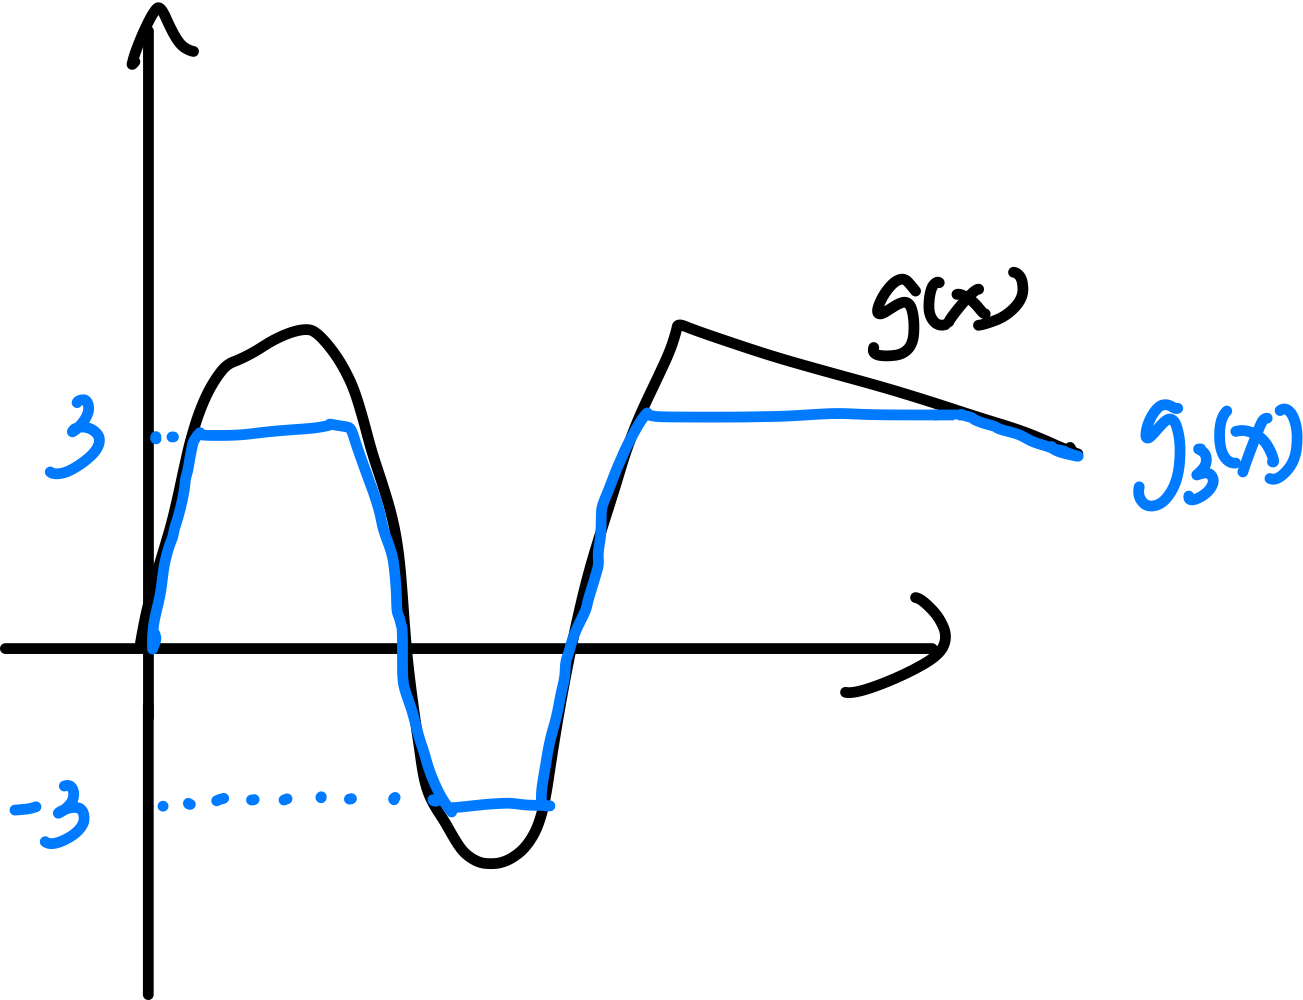
\includegraphics[width=0.35\linewidth,height=\textheight,keepaspectratio]{assets/main--figure-raster-014.png}

\end{center}

\textbf{proof of remaining:} Therefore we have:

\[E = \bigcup\limits_{N = 1}^{\infty}\bigcap\limits_{n \geq N}\left\{ {x \in X \mid g_{n}(x) = h_{n}(x)} \right\}\]

Foe each \(n \in {\mathbb{N}}\), we define

\[E_{n} := \left\{ {x \in X \mid g_{n}(x) = h_{n}(x)} \right\}\]

Since each \(g_{n},h_{n}\) is measurable and real-valued (finite), \(g_{n} - h_{n}\) is measurable and \(|g_{n} - h_{n}|\) is measurable, so we have for each \(m \in {\mathbb{N}}\),

\[\left. \left\{ x \in X: \middle| g_{\kappa_{n}}(x) - h_{\kappa_{n}}(x) \middle| < 1/m \right\} = \middle| g_{n} - h_{n} \middle| {}_{- 1}(\lbrack 0,1/m)) \in \mathcal{A} \right.\]

Thus

\[\left. E_{n} = \bigcap\limits_{m \in {\mathbb{N}}} \middle| g_{n} - h_{n} \middle| {}_{- 1}(\lbrack 0,1/m)) \in \mathcal{A} \right.\]

is a measurable set. Thus \(E\) is a countable union of countable intersections of mea surable sets, then measurable.

\end{proof}

\begin{proof}

\textbf{of method (ii):}\\
Recall: \textbf{a seq of real numbers converges iff it is a Cauchy.} Now we fix an arbitrary \(i \in {\mathbb{N}}\) and let \(\epsilon = 1/i\). Define:

\[E_{i,j,k} = \left\{ x \in X: \middle| f_{j}(x) - f_{k}(x) \middle| < 1/i \right\}\]

Since each \(f_{j}\) is measurable, the function \(\left. x\mapsto \middle| f_{j}(x) - f_{k}(x)| \right.\) is measurable (since each term in the sequence maps to \(\mathbb{R}\) but not \(\bar{\mathbb{R}}\)), and hence \textbf{each \(\left. E_{i,j,k} = \middle| f_{j}(x) - f_{k}(x) \middle| {}_{- 1}(\lbrack 0,1/i)) \right.\) is measurable.}\\
\strut \\
For each \(i\), consider the set of \(x \in X\) for which the sequence \((f_{n}(x))\) satisfies the Cauchy condition with respect to \(\epsilon = 1/i\). That is,

\[E_{i} = \left\{ x \in X:\exists N \in {\mathbb{N}}\ \text{s.t.}\ \forall j,k \geq N, \middle| f_{j}(x) - f_{k}(x) \middle| < \frac{1}{i} \right\}\]

We can write \(E_{i}\) as

\[E_{i} = \bigcup\limits_{N = 1}^{\infty}\bigcap\limits_{j,k \geq N}E_{i,j,k}\]

Since countable unions and intersections of measurable sets are measurable, \textbf{\(E_{i}\) is measurable.}\\
\strut \\
Now, since \((f_{n}(x))\) converges in \(\mathbb{R}\) i\textbf{ff it is Cauchy, i.e. it is in \(E_{i}\) for each \(i \in {\mathbb{N}}\)}, we have:

\[E = \bigcap\limits_{i = 1}^{\infty}E_{i} = \bigcap\limits_{i = 1}^{\infty}(\bigcup\limits_{N = 1}^{\infty}\bigcap\limits_{j,k \geq N}E_{i,j,k})\]

This is a countable intersection of measurable sets, and therefore \(E\) is measurable.

\end{proof}

\section{Measurability of continuity loci.}

Let \((X,d)\) be a metric space, and \(f:X\rightarrow{\mathbb{C}}\) any function. Prove that the set of points \(x \in X\) such that \(f\) is continuous at \(x\) is a \(G_{\delta}\)-set, and in particular a Borel set. \emph{Hint}: consider sets of the form

\[\left\{ x \in X \mid \middle| f(y) - f(z) \middle| \leq \frac{1}{n}\ \text{whenever}\max\left\{ {d(y,x),d(z,x)} \right\} \leq \delta \right\}\]

and show off your skills with quantifiers.

\begin{proof}

Recall: \(f:X\rightarrow{\mathbb{C}}\) \textbf{from a metric space} is continuous at \(x \in X\) iff for every \(\varepsilon > 0\) there exists a \(\delta > 0\) such that\(\left. |f(y) - f(x) \middle| < \varepsilon\ \text{whenever}\ d(y,x) < \delta \right.\). We can easily check that, \textbf{this condition is equivalent to}: for every \(\varepsilon > 0\) there exists a \(\delta > 0\) such that \(\left. |f(y) - f(z) \middle| < \varepsilon\quad\forall y,z \in B_{\delta}(x) \right.\), by the relation of diameter and radius of the open ball).\\
\strut \\
Thus we have:

\[\left. x \in C\Leftrightarrow\forall n \in {\mathbb{N}},\ \exists m \in {\mathbb{N}}\ \text{s.t.}\ y,z\ \text{with}\ d(y,x) < \frac{1}{m}\ \text{and}\ d(z,x) < \frac{1}{m}, \middle| f(y) - f(z) \middle| < \frac{1}{n} \right.\]

In other words, \textbf{\(x\) is a continuity point iff it belongs to:}

\[C = \bigcap\limits_{n = 1}^{\infty}\bigcup\limits_{m = 1}^{\infty}U_{n,m}.\]

where

\[U_{n,m} = \left\{ x \in X \mid y,z \in B_{\frac{1}{m}}(x)\Longrightarrow \middle| f(y) - f(z) \middle| < \frac{1}{n} \right\}\]

\textbf{Claim: \(U_{n,m}\) is open.}\\
\textbf{Proof of Claim:}\\
Let \(x \in U_{n,m}\). WTS: \(\exists\) an \(\varepsilon > 0\) such that \(B_{\varepsilon}(x) \subset U_{n,m}\).\\
Consider: \(\varepsilon = \frac{1}{2m}\).\\
Let \(y \in B_{\varepsilon}(x)\). Take any two points \(z,w \in X\) satisfying

\[d(z,y) < \frac{1}{2m}\quad\text{and}\quad d(w,y) < \frac{1}{2m}\]

Then by the triangle inequality, we have:

\[d(z,x) \leq d(z,y) + d(y,x) < \frac{1}{2m} + \frac{1}{2m} = \frac{1}{m}\]

Similarly, \(d(w,x) < \frac{1}{m}\). Since \(x \in U_{n,m}\), it follows that

\[\left. |f(z) - f(w) \middle| < \frac{1}{n} \right.\]

Thus, the condition defining \(U_{n,m}\) holds for \(y\), meaning \(y \in U_{n,m}\). This proves that \(B_{\varepsilon}(x) \subset U_{n,m}\), thus \(U_{n,m}\) is open since \(x\) is arbitrary.\\
\strut \\
Therefore:

\[C = \bigcap\limits_{n = 1}^{\infty}\bigcup\limits_{m = 1}^{\infty}U_{n,m}\]

is \(G_{\delta}\) since each \(\bigcup_{m = 1}^{\infty}U_{n,m}\) is a union of open sets, thus open; and \(C\) is thus a countable intersection of open sets, namely a \(G_{\delta}\)-set. (thus Borel).

\end{proof}

\section{Measurability of differentiability loci.}

Let \(f:{\mathbb{R}}\rightarrow{\mathbb{R}}\) be any function. Let us say (as usual) that \(f\) is \textbf{\emph{differentiable}} at \(x\) if there exists \(\lambda \in {\mathbb{R}}\) such that \(\lim_{y\rightarrow x}\frac{f(y) - f(x)}{y - x} = \lambda\).

We also declare \(f\) to be \textbf{\emph{strongly differentiable}} at \(x\) if there exists \(\lambda \in {\mathbb{R}}\) with the following property: for each \(\epsilon > 0\) there exists \(\delta > 0\) such that if \(\left. |y - x \middle| \leq \delta \right.\) and \(\left. |z - x \middle| \leq \delta \right.\), then \(\left. |f(y) - f(z) - \lambda(y - z) \middle| \leq \epsilon \middle| y - z| \right.\).

\begin{itemize}
\item
  Does \(f\) being differentiable at \(x\) imply that \(f\) is strongly differentiable at \(x\)? Give a proof or a counterexample.
\item
  Prove that the set of points \(x \in {\mathbb{R}}\) at which \(f\) is strongly differentiable is a Borel set. \emph{Hint}: consider sets of the form

  \[\left. E_{\lambda,m,n} := \{ x \in {\mathbb{R}} \mid \middle| f(y) - f(z) - \lambda(y - z) \middle| \leq \frac{1}{n} \middle| y - z \middle| \ \text{whenever}\max\left\{ |y - x \middle| , \middle| z - x \middle| \leq \frac{1}{m} \right\}. \right.\]
\item
  \emph{Extra credit}: is the set of points \(x \in {\mathbb{R}}\) at which \(f\) is differentiable a Borel set?
\end{itemize}

\begin{qlsolution}{Solution}

\textbf{of (a):} No. Consider the following counterexample:\\

\[f(x) = \left\{ \begin{matrix}
{x^{2}\sin(\frac{1}{x}),} & {x \neq 0} \\
{0,} & {x = 0}
\end{matrix} \right.\]

We know that

\[\frac{f(x) - f(0)}{x - 0} = \frac{x^{2}\sin(1/x)}{x} = x\sin(1/x)\]

Note \(\left. |x\sin(1/x) \middle| \leq \middle| x| \right.\), so when \(x\rightarrow 0\) we have:

\[\lim\limits_{x\rightarrow 0}x\sin(1/x) = 0\]

Thus \(f\) is differentiable at \(0\) and \(f'(0) = 0\).

% qlnotes: kind=lemma; id=lem-hw04-on-measurable-functions-lemma-001; concepts=lemma-001
\begin{lemma}\label{lem-hw04-on-measurable-functions-lemma-001}

\(f:{\mathbb{R}}\rightarrow{\mathbb{R}}\) is strongly differentiable at \(x\) \(\Longrightarrow\) it is differentiable at \(x\), and \(\lambda\) is uniquely equal to the derivative at \(x\).

\end{lemma}

\begin{proof}

\textbf{of lemma 4.1:}\\
Suppose \(f:{\mathbb{R}}\rightarrow{\mathbb{R}}\) is strongly differentiable at \(x\), so for any \(\epsilon > 0\), there exists \(\delta > 0\) s.t. for all \(y,z \in B_{\delta}(x)\), we have:

\[\left. |\ f(y) - f(z) - \lambda(y - z) \middle| \leq \epsilon\, \middle| y - z \middle| . \right.\]

Suppose \(y \neq z\), then dividing by \(|y - z|\) on both sides, we have

\[\left. |\ \frac{f(y) - f(x)}{y - x} - \lambda\  \middle| \leq \epsilon \right.\]

Since \(\epsilon\) is arbitrary, this proves that

\[f'(x) = \lim\limits_{y\rightarrow x}\frac{f(y) - f(x)}{y - x} = \lambda\]

\end{proof}

Now we go back to the counterexample. Suppose for contradiction that \(f\) is strongly differentiable at \(0\), then \(\lambda = 0\), so for all \(\epsilon > 0\), there exist \(\delta > 0\) s.t. for all \(y,z \in B_{\delta}(0)\), we have

\[\left. |f(y) - f(z) \middle| \leq \epsilon\, \middle| y - z| \right.\]

Consider \(\epsilon = \frac{1}{4}\). Let \(\delta > 0\). Take \(n \in {\mathbb{N}}\) s.t.

\[\frac{1}{(2n + \frac{3}{2})\pi} < \delta\]

and then take

\[y_{n} := \frac{1}{\left( {2n + \frac{1}{2}} \right)\pi},\quad z_{n} := \frac{1}{\left( {2n + \frac{3}{2}} \right)\pi}\]

Note that each \(\left. |y_{n} \middle| , \middle| z_{n} \middle| < \delta \right.\). And we have

\[\sin\lbrack(2n + \frac{1}{2})\pi\rbrack = ( - 1)^{n},\quad\sin\lbrack(2n + \frac{3}{2})\pi\rbrack = - ( - 1)^{n}\]

Thus

\[f(y_{n}) - f(z_{n}) = ( - 1)^{n}\lbrack y_{n}^{2} + z_{n}^{2}\rbrack\]

while

\[y_{n} - z_{n} = \frac{1}{\left( {2n + \frac{1}{2}} \right)\pi} - \frac{1}{\left( {2n + \frac{3}{2}} \right)\pi} = \frac{1}{\pi\left( {2n + \frac{1}{2}} \right)\left( {2n + \frac{3}{2}} \right)}\]

Taking limit of this behavior (increasing \(n\)), we get the sequential limit of \(\frac{|f(y_{n}) - f(z_{n})|}{|y_{n} - z_{n}|}\) indexing over \(n\) is \(\frac{\frac{1}{2\pi^{2}n^{2}}}{\frac{1}{4\pi n^{2}}} = \frac{2}{\pi}\). By taking large enough \(n\), we can alwasy get \(\frac{|f(y_{n}) - f(z_{n})|}{|y_{n} - z_{n}|}\) to be arbitrarily close to \(\frac{2}{\pi} > \frac{1}{4}\). This shows that \(f\) is not strongly differentiable at \(0\).

\end{qlsolution}

\begin{proof}

\textbf{of (b):}\\
Let \(f:{\mathbb{R}}\rightarrow{\mathbb{R}}\) be any a function.Denote

\[E: = \left\{ {x \in {\mathbb{R}} \mid f\ \text{is strongly differentiable at}\ x} \right\}\]

WTS: \(E\) is a Borel set.

Set for each \(\lambda \in {\mathbb{R}},m,n \in {\mathbb{N}}\):

\[E_{\lambda,m,n} := \left\{ x \in {\mathbb{R}} \mid \middle| f(y) - f(z) - \lambda(y - z) \middle| \leq \frac{1}{n} \middle| y - z \middle| \ \forall y,z \in B_{\frac{1}{m}}(x) \right\}\]

where \(B_{\frac{1}{m}}(x)\) denote the open ball centered at \(x\) with radius \(\frac{1}{m}\).

Then by the definition of strongly differentiable, we have:

\[E = \bigcup\limits_{\lambda \in {\mathbb{R}}}\bigcap\limits_{n \in {\mathbb{N}}}\bigcup\limits_{m \in {\mathbb{N}}}E_{\lambda,m,n}\,\]

\textbf{Claim 3.1: Each \(E_{\lambda,m,n}\) is open.}\\
\textbf{Proof of Claim 3.1:} Let \(x \in E_{\lambda,m,n}\). Then

\[\left. \forall y,z \in B_{1/m}(x),\quad \middle| \ f(y) - f(z) - \lambda(y - z) \middle| \leq \frac{1}{n}\, \middle| y - z| \right.\]

In particular, the inequality holds for all \(y,z \in B_{1/(2m)}(x)\). Now consider \(B_{1/(2m)}(x)\), let \(x' \in B_{1/(2m)}(x)\), then for every \(y \in B_{1/(2m)}(x')\), we have

\[\left. |y - x \middle| \leq \middle| y - x' \middle| + \middle| x' - x \middle| < \frac{1}{2m} + \frac{1}{2m} = \frac{1}{m} \right.\]

so \(B_{1/(2m)}(x') \subset B_{1/m}(x)\). Hence the inequality holds for all \(y,z \in B_{1/(2m)}(x')\). This confirms that every \(x \in E_{\lambda,m,n}\) has a neighborhood contained in \(E_{\lambda,m,n}\), proving that \(E_{\lambda,m,n}\) is open.\\
\strut \\
Now that each \(E_{\lambda,m,n}\) is open, we have \(\bigcup_{m \in {\mathbb{N}}}E_{\lambda,m,n}\) is each for each \(\lambda,n\); thus each for each \(\lambda\), \(\ G_{\lambda} := \bigcap_{n \in {\mathbb{N}}}\bigcup_{m \in {\mathbb{N}}}E_{\lambda,m,n}\) is a \(G_{\delta}\) set.

\[E = \bigcup\limits_{\lambda \in {\mathbb{R}}}G_{\lambda}\]

is a union of \(G_{\delta}\) sets.

(I do not now how to deal with it then, it might be that we somehow reduce it to countable union of \(G_{\delta}\) sets, getting something like \(E = \bigcup_{\lambda \in {\mathbb{Q}}}G_{\lambda}\) using the density of \(\mathbb{Q}\) in \(\mathbb{R}\), thus confirming that it is Borel.) -2. 这里的正解是: 要利用 density of \(\mathbb{Q}\) in \(\mathbb{R}\) 的话, 只需要考虑交换 set operation 的顺序就好了. 我们会发现其实:

\[E = \bigcap\limits_{n \in {\mathbb{N}}}\bigcup\limits_{\lambda \in {\mathbb{Q}}}\bigcup\limits_{m \in {\mathbb{N}}}E_{\lambda,m,n}\,\]

就这么简单。。

\end{proof}

\begin{proof}

of extra credit: yes. 这个解法非常麻烦. 需要再多考虑两层. 令 \(E_{\lambda,k,l,m,n}\) 表示 the set of points \(x\) s.t.

\[\left. |f(y) - f(z) - \lambda(y - z) \middle| \leq \frac{1}{n} \middle| y - z| \right.\]

whenever

\[\left. \frac{1}{2^{l + 1}}(1 + \frac{1}{2^{k}}) \leq \middle| y - x \middle| \leq \frac{1}{2^{l - 1}}(1 - \frac{1}{2^{k}})\quad\text{and}\quad \middle| z - x \middle| \leq \frac{1}{2^{m}}(1 - \frac{1}{2^{k}}) \right.\]

Claim:

\[f\ \text{is differentiable at x}\ \text{iff}\ x \in E := \bigcap\limits_{n \in {\mathbb{N}}}\bigcup\limits_{\lambda \in {\mathbb{Q}}}\bigcup\limits_{l \in {\mathbb{N}}}\bigcap\limits_{r \geq l}\bigcup\limits_{m \geq 1}\bigcup\limits_{k \in {\mathbb{N}}}E_{\lambda,k,r,m,n}\]

\end{proof}

\section{decreasing MCT: 成立当且仅当 integral 的 limit 是 finite 的}\label{decreasing-mct-ux6210ux7acbux5f53ux4e14ux4ec5ux5f53-integral-ux7684-limit-ux662f-finite-ux7684}

Let \((f_{n})_{1}^{\infty}\) be a \emph{decreasing} sequence of non-negative measurable functions on a measure space.

\begin{itemize}
\item
  Prove that if \(\lim_{n}\int f_{n} < \infty\), then \(\lim_{n}\int f_{n} = \int\lim_{n}f_{n}\).
\item
  Give an example of a decreasing sequence \((f_{n})_{n}\) of nonnegative measurable functions such that \(\lim_{n}\int f_{n} \neq \int\lim_{n}f_{n}\).
\end{itemize}

\emph{Hint}: use MCT correctly.

\begin{proof}

\textbf{of (a):}\\
Since \((f_{n})\) is a decreasing sequence, i.e. for every \(x \in X\) we have

\[f_{1}(x) \geq f_{2}(x) \geq f_{3}(x) \geq \cdots\]

We can define the function

\[g_{n}(x) = f_{1}(x) - f_{n}(x)\]

for each \(n \in {\mathbb{N}}\). Then for the seq \((g_{n}(x))\) we have:

\begin{itemize}
\item
  non-negatice: \(g_{n}(x) \geq 0\forall x\) because \(f_{1}(x) \geq f_{n}(x)\).
\item
  increasing in \(n\):

  \[g_{n}(x) = f_{1}(x) - f_{n}(x) \leq f_{1}(x) - f_{m}(x) = g_{m}(x)\forall m \geq n,\forall x\]

  since \((f_{n})\) is decreasing.\\
  \strut \\
\end{itemize}

Define \(f(x) := \lim_{n}f_{n}(x) \in \bar{\mathbb{R}}\) for each \(x \in X\).

Since \(f_{n}(x)\) decreases to \(f(x) := \lim_{n\rightarrow\infty}f_{n}(x)\), we have

\[\lim\limits_{n\rightarrow\infty}g_{n}(x) = f_{1}(x) - \lim\limits_{n\rightarrow\infty}f_{n}(x) = f_{1}(x) - f(x)\]

Now we \textbf{apply MCT to the increasing sequence \((g_{n})\)}. We have:

\[\lim\limits_{n\rightarrow\infty}\int g_{n}\, d\mu = \int(\lim\limits_{n\rightarrow\infty}g_{n})\, d\mu = \int(f_{1} - f)\, d\mu\]

And since \(\lim_{n\rightarrow\infty}\int f_{n}\, d\mu < \infty\), we have

\[\lim\limits_{n\rightarrow\infty}\int g_{n}\, d\mu = \int f_{1}\, d\mu - \int f d\mu\]

Also, because of \(\lim_{n\rightarrow\infty}\int f_{n}\, d\mu < \infty\), \textbf{\(\int f_{n}\) is eventually finite}. Say, it is finite after \(n \geq N \in {\mathbb{N}}\). We only need to consider \(n \geq N\) when considering the limit behavior.\\
Then for each \(n \geq N\),

\[\int g_{n}\, d\mu = \int(f_{1} - f_{n})\, d\mu = \int f_{1}\, d\mu - \int f_{n}\, d\mu\]

-2. 这里注意, 我们既然知道 \(f_{1}\) 的 integral 未必 finite, 就不能这么定义 \(g_{n}\). 正解是取 \(N\) s.t. \(\int f_{N}\) finite, 然后定义 \(g_{n} := f_{N} - f_{n}\). Taking the limit as \(n\rightarrow\infty\), have

\[\lim\limits_{n\rightarrow\infty}\int g_{n}\, d\mu = \lim\limits_{n\rightarrow\infty}\left( {\int f_{1}\, d\mu - \int f_{n}\, d\mu} \right) = \int f_{1}\, d\mu - \lim\limits_{n\rightarrow\infty}\int f_{n}\, d\mu\]

by linearity of numerical sequence.\\
Thus, combining with the result from MCT we have:

\[\int f_{1}\, d\mu - \lim\limits_{n\rightarrow\infty}\int f_{n}\, d\mu = \int f_{1}\, d\mu - \int f d\mu\]

Rearrange to get:

\[\lim\limits_{n\rightarrow\infty}\int f_{n}\, d\mu = \int f\, d\mu,\]

which is exactly what we wanted to prove.

\end{proof}

\begin{qlsolution}{Solution}

\textbf{of (b):}\\
Consider defining \((f_{n}:{\mathbb{R}}\rightarrow{\mathbb{R}})_{n \in {\mathbb{N}}}\) with

\[f_{n}(x) = \chi_{\lbrack n,\infty)}(x)\]

Note that:

\begin{itemize}
\item
  \textbf{\(f_{n}\) is a decreasing seq}: For each \(n\) and every \(x \in {\mathbb{R}}\),

  \[f_{n + 1}(x) = \chi_{\lbrack n + 1,\infty)}(x) \leq \chi_{\lbrack n,\infty)}(x) = f_{n}(x)\]

  since \(\lbrack n + 1,\infty) \subset \lbrack n,\infty)\).
\item
  \textbf{\((f_{n})\) the pointwise limit}:

  \[\lim\limits_{n\rightarrow\infty}f_{n}(x) = 0\quad\forall x \in {\mathbb{R}}\]

  since for each \(x\) there exists an \(N\) (any integer greater than \(x\)) such that for all \(n \geq N\), \(x < n\) and hence \(f_{n}(x) = 0\).
\item
  For each \(n\),

  \[\int_{\mathbb{R}}f_{n}\, d\lambda = \int_{n}^{\infty}1\, dx = \infty\]

  But on the other hand

  \[\int_{\mathbb{R}}(\lim\limits_{n\rightarrow\infty}f_{n})\, d\lambda = \int_{\mathbb{R}}0\, d\lambda = 0\]
\end{itemize}

Then we have the decreasing seq of function with

\[\lim\limits_{n\rightarrow\infty}\int f_{n}\, d\lambda = \infty\quad\text{while}\quad\int(\lim\limits_{n\rightarrow\infty}f_{n})\, d\lambda = 0\]

This shows that in the absence of the finiteness assumption, the limit and integration need not commute.

\end{qlsolution}

\section{Vitali meet Cantor.}

Construct a function \(f:\lbrack 0,1\rbrack\rightarrow\lbrack 0,1\rbrack\) such that:

\begin{itemize}
\item
  \(f\) fails to be Lebesgue measurable;
\item
  there exists a compact subset \(K \subset (0,1)\) of positive Lebesgue measure such that \(f\) is differentiable at every point \(x \in K\).
\end{itemize}

\emph{Hint}: use the function \(g(x) = \inf\left\{ |x - y \middle| \mid y \in K \right\}\); then square this with the title of the problem.

\begin{qlsolution}{Solution}

Let \(V\) be a Vitali set on \(\lbrack 0,1\rbrack\), \(C\) be the fat Cantor set on \(\lbrack 0,1\rbrack\) by recursively taking away the middle open subinterval of length \(\frac{1}{4^{n}}\) on the \(n\)th recursion. We consider the function:

\[f(x) = \chi_{V} \cdot d(x,C)^{2}\]

where

\[d(x,C) := \{\inf\left\{ |x - y \middle| \mid y \in C \right\}\]

By Hw3, we know \(V\) is not Lebesgue measurable, and \(C\) is compact with positive Lebesgue measure \(\frac{1}{2}\).

And since \(f^{- 1}(\left\{ 1 \right\}) = V\), mapping a not measurable set to a measurable set, \textbf{\(\chi_{V}\) is not measurable function.}

And since the distance function \(d(x,C)\) is a continuous function of \(\lbrack 0,1\rbrack\), it is measurable, by the result proved in class that a continuous funciton on a topological space is measurable.

% qlnotes: kind=lemma; id=lem-hw04-on-measurable-functions-lemma-002; concepts=lemma-002
\begin{lemma}\label{lem-hw04-on-measurable-functions-lemma-002}

The product of a measurable \(f:{\mathbb{R}}\rightarrow{\mathbb{R}}_{> 0}\) and a not measurable \(g:{\mathbb{R}}\rightarrow{\mathbb{R}}\) is not measurable.

\end{lemma}

\textbf{Proof of Lemma 4.2:} \(f\) measurable \(\Longrightarrow\) \(1/f\) measurable. Suppose for contradiction that \(fg\) is measurable, then \(g = \frac{1}{f}(fg)\) is the product of two measurable functions, thus measurable, contradicting the fact that \(g\) is not measurable. Thus \(fg\) is not measurable.\\
\strut \\
\textbf{Claim 5.1: \(f\) is not measurable.} \textbf{Proof of claim 5.1:} Thus on the open set \(A = \lbrack 0,1\rbrack\backslash C\), \(d(x,C)^{2}\) is positive, so \(\left. \chi_{V} \middle| {}_{A}\ d(x,C)^{2}|_{A} \right.\) is not measurable since it is a product of measurable and not measurable function by lemma 4.2. Thus \textbf{\(f\) is not measurable,} otherwise its restriction on \(A\) should also be measurable.\\
\strut \\
\textbf{Claim 5.2: \(f\) is differentiable on \(C\).} \textbf{Proof of claim 5.2:} Fix \(x \in C\), then \(f(x) = 0\). We want to show:\(f'(x) = \lim_{h\rightarrow 0}\frac{f(x + h) - f(x)}{h} = \lim_{h\rightarrow 0}\frac{f(x + h)}{h}\) exists Let \(h > 0\). Case 1: \(x + h \notin V\), then \(\chi_{V}(x + h) = 0\), so we have \(f(x + h) = \chi_{V}(x + h)\, d(x + h,C)^{2} = 0\), then \(\frac{f(x + h)}{h} = 0\). Case 2: \(x + h \in V\), we have:

\[\left. d(x + h,C) = \inf\limits_{y \in C} \middle| (x + h) - y \middle| \leq \middle| (x + h) - x \middle| = \middle| h| \right.\]

So

\[\left. \left| \frac{f(x + h)}{h} \right| = \frac{d(x + h,C)^{2}}{|h|} \leq \frac{|h|^{2}}{|h|} = \middle| h| \right.\]

Therefore for all cases we have:

\[\left. \left| \frac{f(x + h) - f(x)}{h} \right| = \left| \frac{f(x + h)}{h} \right| \leq \middle| h| \right.\]

This confirms that

\[f'(x) = \lim\limits_{h\rightarrow 0}\frac{f(x + h) - f(x)}{h} = 0\]

This finishes the proof of required properties of \(f\).

\end{qlsolution}

\subsection{harder Vitali meet Cantor (extra credit)}\label{harder-vitali-meet-cantor-extra-credit}

We change the requirement of (a) to be: "the restriction of \(f\) to any open interval \(I \subset \lbrack 0,1\rbrack\) fails to be Lebesgue measurable". Then how can we make the construction?

\begin{qlsolution}{Solution}

I don't know.\\
官方答案: 我在前一问给出的

\[f(x) = \chi_{V} \cdot d(x,C)^{2}\]

这个函数, 同样也是满足这一问的答案. (对于 \(C\), 不仅可以选择 fat Cantor set, 实际上任何 choice of compact nowhere dense set 都可以.)

\end{qlsolution}
\end{document}
